\begin{figure*}[t]
  \centering
  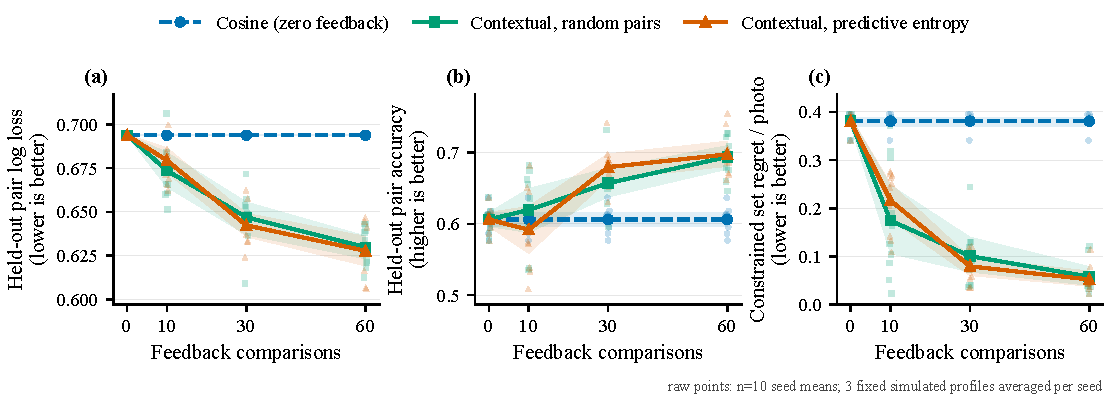
\includegraphics[width=0.95\textwidth]{figures/fig3_contextual_preference_learning.pdf}
  \caption{Learning curves for the 67D contextual preference adapter on 70 public Wikimedia images under three declared category-utility simulators. Each replicate uses a category-stratified exact-file-disjoint 42/28 train/test split. Lines are means across 10 split/choice seeds after averaging three fixed simulated profiles per seed; shaded regions are 95\% percentile-bootstrap intervals over seed means and faint points are the raw seed means. At 60 feedback comparisons, all paired predictive-entropy-versus-random intervals cross zero, so the curves do not establish superiority of entropy acquisition. The experiment uses no human preferences and does not establish population generalization.}
  \label{fig:controlled-contextual-preference}
\end{figure*}
